% Niveau :      PCSI
% Discipline :  Mécaflu
%Mots clés :    

\begin{exercise}{Fréquence de Brunt--Väisälä}{2}{Sup, Spé}
{Statique des fluides}{bermu}

Dans cet exercice, on considère un fluide dit stratifié, ayant des profils de densité et de pression $\rho(z)$, $P(z)$, $z$ étant l'altitude, sous un profil de gravité uniforme $\vec{g} = -g\ve_z$. On étudie la dynamique d'un petit cube de taille $a$ de ce fluide, dont on repère l'altitude par la variable $\xi$.

\begin{questions}
    \questioncours \'Etablir l'équation différentielle vérifiée par $\xi$ et redémontrer l'équation de la statique des fluides. 
    \uplevel{On suppose par la suite que le fluide est globalement à l'équilibre hydrostatique.
    
    Le cube, initialement à l'altitude $\xi = 0$ et de densité $\rho(0) = \rho_0$, est élevé à une altitude $\xi > 0$, sans dilatation.}
    \question \'Etablir l'équation différentielle vérifiée par $\xi$. Quelle forme classique prend-t-elle ? Montrer que suivant une condition sur $\dv{\rho}{z}$, la stratification du fluide est stable, ou instable.
    \question Quel est le comportement du cube dans le cas d'une stratification stable ? Introduire une fréquence typique, notée $N$, la fréquence de Brunt--Väisälä. 
    \begin{EnvUplevel} On se propose d'étudier un tel exemple avec la photographie suivante :
    \begin{figure}[H]
        \centering
        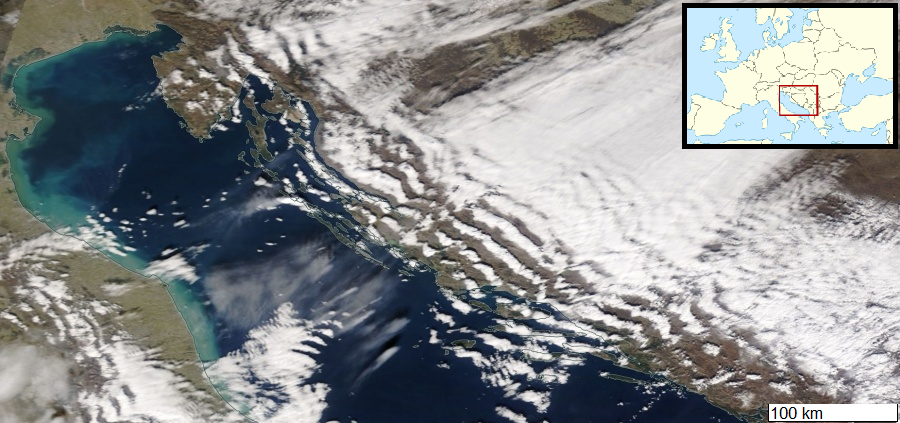
\includegraphics[width=\linewidth]{mecaflu/statiqueflu/gravity_waves.png}
        \caption{Ondes internes photographiées au large de la mer Adriatique le 25/02/2019. \newline Elles sont formées par la rencontre d'un courant d'air de haute altitude avec les Alpes dinariques dans les Balkans (Slovénie, Croatie, Bosnie, Serbie...)}
    \end{figure}
    \end{EnvUplevel}
    \question Estimer la longueur d'onde de cette onde. En déduire à l'aide des données météorologiques la fréquence associée.
    \question En utilisant la relation des gaz parfaits, en déduire une estimation du gradient thermique $\dv{T}{z}$ en $\SI{}{K/km}$.
\end{questions}

\paragraph{Données :}
\begin{itemize}
    \item accélération de la pesanteur terrestre $g = 9,81$ m$^2\cdot$s$^{-1}$,
    \item constante des gaz parfaits $R = 8,314$ $\mathrm{J\cdot mol^{-1}\cdot m^{-3}}$,
    \item pour l'air $M = 28,9$ g$\cdot$mol$^{-1}$
    \item extrait du bulletin météorologique marine du 25/02/2019 dans l'Adriatique nord : \\
    \texttt{VENTS : haute altitude ($> \SI{3000}{m}$), Nord-Est, 60 noeuds ($\SI{30}{m/s}$), température $\SI{297}{K}$.}

\end{itemize}
\end{exercise}

\begin{solution}

\begin{questions}
    \questioncours Bilan des forces : gravité $-\rho(\xi) a^3 g$, pression : $a^2 \qty\big(P(\xi-a/2) - P(\xi+a/2)) \simeq -a^3\eval{\dv{P}{z}}_\xi $. Ainsi
    $$\rho(\xi) \ddot{\xi} = - \rho(\xi) g - \eval{\dv{P}{z}}_\xi \qqtext{soit en statique} \pdv{P}{z} = -\rho g$$
    \question Ainsi en pas statique
    $$\rho(0) \ddot{\xi} = - \rho(0) g - \eval{\dv{P}{z}}_\xi = g\qty\big(\rho(\xi) - \rho(0)) \simeq g \dv{\rho}{z} \xi$$
    soit
    $$\ddot{\xi} -\dfrac{g}{\rho_0}\dv{\rho}{z}\xi = 0$$
    On a une équation d'oscillateur harmonique si $\dv{\rho}{z} < 0$ $=$ stratifié stable, le mouvement oscille. Sinon on diverge.
    \question Le cube oscille à une fréquence $N = \sqrt{-\dfrac{g}{\rho_0}\dv{\rho}{z}}$
    \question $\lambda = \SI{16}{km}$. Ainsi si $v =\SI{30}{m/s}$, $f = v/\lambda = \SI{2e-3}{s^{-1}}$
    \question $N^2 = -\dfrac{g}{\rho_0}\dv{\rho}{z}$ et $P_0 M = \rho R T_0$ donne $N^2 = -\dfrac{g}{T_0}\dv{T}{z}$. Donc $\dv{T}{z} = \SI{0.1}{K/km}$.
\end{questions}

Plus : \url{https://www.atmos.millersville.edu/~adecaria/ESCI342/ANSWERS/esci342_exercises_answers_lesson09.html}

\end{solution}